% Created 2025-06-13 Fri 11:48
% Intended LaTeX compiler: pdflatex
\documentclass[bigger,aspectratio=169]{beamer}
 \usepackage{minted}
 \usepackage{caption, subcaption, csquotes, amssymb, xcolor}
\usepackage[english]{babel}
\titlegraphic{\includesvg[height=1cm]{./figs/IE_Unicamp}\hspace*{1.25cm}\includesvg[height=1cm]{./figs/SSSA}\hspace*{1.25cm} \includesvg[height=1cm]{./figs/YSI}}
\AtBeginSection[]{
\begin{frame}{Outline}
\tableofcontents[currentsection]
\end{frame}
}
\usepackage[utf8]{inputenc}
\usepackage[T1]{fontenc}
\usepackage{amsmath}
\usepackage{amsfonts}
\usepackage{amssymb}
\usepackage{multicol}
\usepackage{graphicx}
\usepackage{textpos}
\usepackage{caption}
\usepackage{subfig}
\usepackage{svg}
\usepackage{pgfpages}
\usepackage{epstopdf}
\epstopdfsetup{update} % only regenerate if changed
\DeclareGraphicsRule{.eps}{pdf}{.pdf}{`epstopdf #1}
\usepackage{minted}
\setminted{autogobble,fontsize=\footnotesize}
\usemintedstyle{perldoc}
\usepackage{tikz}
\usetikzlibrary{arrows.meta, positioning, shapes}
\usepackage{fontawesome5}
\usetheme{Pittsburgh}
\usecolortheme{beaver}
\author{Gabriel Petrini}
\date{July, 2025}
\title{ABM Macro Lab: Agent-based Modelling Tools}
\subtitle{Coding session}
\usepackage[style=authoryear]{biblatex}
\addbibresource{~/Org/zotero_refs.bib}
\begin{document}

\maketitle
\begin{frame}{Outline}
\tableofcontents
\end{frame}

\section{Introduction}
\label{sec:org52c243f}

\begin{frame}[label={sec:org2acfe90}]{Objectives}
Throughout the sessions, we will

\begin{enumerate}
\item Understand how LSD works.
\item Implement a linear and a chaotic model\footnote{Based on the slides of LSD manual folder}
\item Understand and implement the \textcite{dosi_2017_footprint} model on LSD
\item Analyze the model results on LSD
\end{enumerate}
\end{frame}
\begin{frame}[label={sec:orgc32d983}]{Structure of the sessions}
\begin{description}
\item[{Session 1}] Presents the general structure of LSD and perform some simulations
\item[{Session 2}] Write the industry model equations in LSD
\item[{Session 3}] Complete the scripts (if necessary), run the simulation and the analysis of results
\item[{Bonus}] A primer on sensitivity analysis
\end{description}
\end{frame}
\begin{frame}[label={sec:orgaf3a216},fragile]{Repository structure}
 This presentation can be found on this \href{https://github.com/gpetrini/CodingSession}{repository}.\footnote{URL: \url{https://github.com/gpetrini/CodingSession}} In addition:

\begin{description}
\item[{Linear\_Model/fun\_linear.cpp}] Starting script for the linear model
\item[{Chaotic\_Model/fun\_chaotic.cpp}] Starting script for the chaotic model
\item[{Industry\_SummerSchool/fun\_industry.cpp}] Starting script for the industry model
\item[{Sim*.lsd}] Are the configuration files
\end{description}

\alert{Important:} Clone/Download this folder under \texttt{LSD/Work/}
\begin{block}{Missed something?}
\texttt{*\_complete.cpp} contains the complete equation file for reference.
\end{block}
\end{frame}
\section{Session 1}
\label{sec:org9ff7e66}

\begin{frame}[label={sec:orgdd658fe},fragile]{C++ for LSD I}
 LSD adds macros to \texttt{C++}.
As a consequence, some basic knowledge on \texttt{C++} is usefull.
What do we need to know here?
\begin{columns}
\begin{column}{0.4\columnwidth}
\begin{block}{In python}
\begin{minted}[]{python}
x = 5 # A comment
y = 2.5
## We do not need to
## work with pointers
\end{minted}
\end{block}
\end{column}
\begin{column}{0.4\columnwidth}
\begin{block}{In C++}
\begin{minted}[]{cpp}
int x = 5; // A comment
double y = 2.5;
object *agent; // Latter
\end{minted}
\end{block}
\end{column}
\end{columns}
\begin{block}{Compilation}
Different from python and R, we need to \alert{compile} our code before using it.
\end{block}
\end{frame}
\begin{frame}[label={sec:org6dba465},fragile]{C++ for LSD II}
 To avoid initializing everything, LSD has some already initialized variables:

\begin{minted}[]{cpp}
v[0] = 10; // We can assing number to
v[1] = 50; // a vector (always available)
T; // Current simulation time
i = 1; // i,h,j,k can be used for integers
cur; cur1; // Pre-allocated pointers
\end{minted}

Those are \alert{local variables} that we can use on equations.
\begin{block}{Debbuging}
LSD has an internal debbuger that allow us to look to local variables on the fly.
\end{block}
\end{frame}
\begin{frame}[label={sec:org928d8d9},fragile]{Macros I}
 \begin{figure}[htbp]
\centering
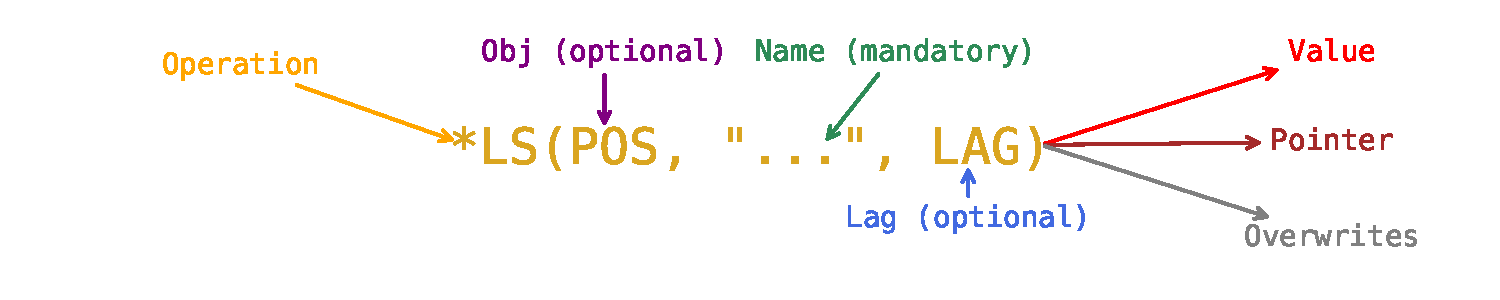
\includegraphics[width=.9\linewidth]{./figs/Macros_LSD.pdf}
\caption{\label{}General structure of most LSD macros}
\end{figure}

Examples:
\begin{description}
\item[{VLS(POS, ``NAME'', 1)}] Returns the value of variable \texttt{NAME} at lag \texttt{1} at position \texttt{POS}
\item[{SUMS(POS, ``NAME'')}] Sums the value of variable \texttt{NAME} at position \texttt{POS}
\item[{SEARCHS(PARENT, ``AGT'')}] Searches for agent \texttt{AGT} starting from \texttt{PARENT}
\item[{WRITELS(POS, ``NAME'', 1)}] Overwrites variable \texttt{NAME} at lag \texttt{1} at position \texttt{POS}
\end{description}
\end{frame}
\begin{frame}[label={sec:org869b2c2}]{Macros II}
\begin{figure}[htbp]
\centering
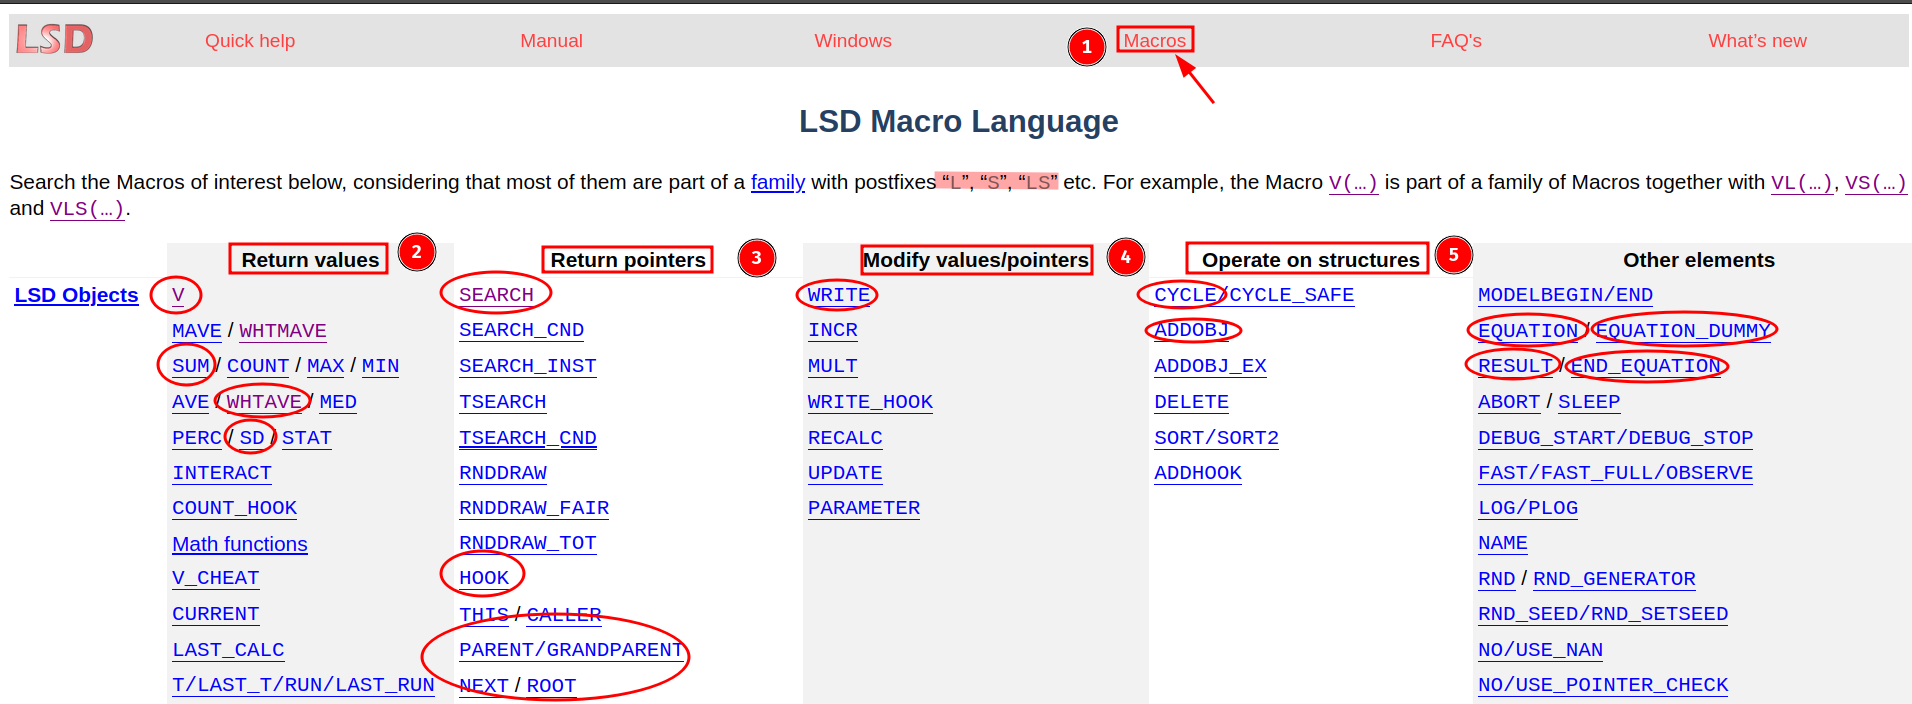
\includegraphics[width=.9\linewidth]{figs/LSD_Macros_ScreenShot.png}
\caption{Other LSD macros}
\end{figure}
\end{frame}
\begin{frame}[label={sec:orgd02ebf4},fragile]{Macro example I}
 How can we write the following equation using LSD syntax?

\[X_{t} = X_{t-1} + m\]

\begin{minted}[]{cpp}
EQUATION("X") // This is a single-line comment
/*
This is a multi-line comment
*/
v[0] = VL("X",1); //past value of X, lagged of 1 period
v[1] = V("m"); //current value of m (variable or parameter)
v[2] = v[0] + v[1]; // v[n] are local variables
RESULT(v[2]) // Specify the output of the function
\end{minted}
\begin{block}{Variable or parameter?}
As a rule of thumb, variables have an \texttt{EQUATION} associated, parameters do not.
\end{block}
\end{frame}
\begin{frame}[label={sec:org722cbb5},fragile]{Macro example II}
 How can we write the following equation using LSD syntax?

\[Y_{t} = \sum_{i=1}^{n} X_{n,t} + W_{n,t-1}\]



\begin{minted}[]{cpp}
EQUATION("Y")
v[0] = 0; // Initialize the Accumulation
CYCLE(cur, "Firm") { // Similar to a for-loop in other languages
    v[1] = VS(cur, "X"); // cur points to a "Firm" object
    v[2] = VLS(cur, "W", 1); // cur is a locally defined pointer
    v[3] = v[1] + v[2];
    v[0] = v[0] + v[3];
}
RESULT(v[0])
\end{minted}
\end{frame}
\begin{frame}[label={sec:org9bcd15e},fragile]{Macro example III}
 We can also write on an alternative way

\[Y_{t} = \sum_{i=1}^{n} X_{n,t} + W_{n,t-1}\]



\begin{minted}[]{cpp}
EQUATION("Y")
// If X and W are bellow Y on the tree (later)
v[0] = SUM("X");
v[1] = SUML("W", 1);
v[2] = v[0] + v[1];
RESULT(v[2])
\end{minted}
\end{frame}
\begin{frame}[label={sec:orga00e2dd},fragile]{Equation file}
 Any equation file (\texttt{.cpp}) must contain the following text:
\begin{minted}[]{cpp}
// File created using org-mode tangle feature.
#include "fun_head.h" // This is mandatory

MODELBEGIN

// Your code goes here

MODELEND
void close_sim(void) {}
\end{minted}

In our session, we will copy-and-paste the initialization equation and continue from there.
\end{frame}
\begin{frame}[label={sec:org135c0f9},fragile]{Model structure and data organization I}
 Besides the equation files (\texttt{.cpp} or \texttt{.h}), LSD defines the model structures on a different file (extension \texttt{.lsd}).
This special file has:

\begin{itemize}
\item Variables and parameters names
\item Model structure (where elements are)
\item Initial and parameter values
\item Simulation settings
\item Number of objects
\item Variables to plot, analyze, debug, etc
\end{itemize}
\begin{block}{LSD and OOP}
This structure ensure the modeler to think in terms of data structure.
\end{block}
\end{frame}
\begin{frame}[label={sec:orge29a142},fragile]{Linear model I}
 Let's start with the file on \url{Linear\_Model/fun\_linear.cpp}


\begin{minted}[]{cpp}
#include "fun_head.h" // This is mandatory

MODELBEGIN

// Your code goes here

MODELEND
void close_sim(void) {}
\end{minted}
\end{frame}
\begin{frame}[label={sec:orge038a3c},fragile]{Linear model II}
 Next, we will write the following equation:

\[X_{t} = X_{t-1} + m\]


\begin{minted}[]{cpp}

EQUATION("X") // This is a single-line comment
/*
This is a multi-line comment
*/
v[0] = VL("X",1); //past value of X, lagged of 1 period
v[1] = V("m"); //current value of m (variable or parameter)
v[2] = v[0] + v[1]; // v[n] are local variables
RESULT(v[2]) // Specify the output of the function
\end{minted}
\end{frame}
\begin{frame}[label={sec:org1577ec6},fragile]{Linear model III}
 \begin{itemize}
\item Compile (\texttt{Model > Compile and run ...}).
\item Wait to open a new window.
\item Create a descending object called \texttt{Obj1} (\texttt{Model > Add Object})
\item Double click on \texttt{Obj1}
\item Add the Variable \(X\) (max. lags = 1, \(X_{0} = 0.5\)) and Parameter (\(m = 2\))
\item Save this configuration as \texttt{Sim1.lsd}
\item Mark \(X\) to be saved (\texttt{F5}) and run
\item Analyze the results
\end{itemize}
\end{frame}
\begin{frame}[label={sec:org010954e}]{Linear model IV}
\begin{center}
\includesvg[width=.83\linewidth]{./figs/Linear_X}
\end{center}
\end{frame}
\begin{frame}[label={sec:org9353286},fragile]{Linear model V}
 We can adjust the previous equation in order to get a Random Walk.
First, we need to specify the distribution for \(m\):

\[m \sim U(\min, \max)\]



\begin{minted}[]{cpp}
EQUATION("m")
v[0] = V("min");
v[1] = V("max");
v[2] = uniform(v[0], v[1]);
RESULT(v[2])
\end{minted}
\end{frame}
\begin{frame}[label={sec:org34d3654},fragile]{Linear model VI}
 Now, we need to adjust the \texttt{.lsd} file:

\begin{itemize}
\item Make a copy of \texttt{Sim1.lsd} and save it as \texttt{Sim2.lsd}
\item \texttt{m} should become an \texttt{EQUATION} on \texttt{.lsd}
\item Create an equation for \texttt{m} (on \texttt{.cpp}) (done)
\item Add new parameters on \texttt{.lsd}
\begin{itemize}
\item \texttt{min} = -10
\item \texttt{max} = 10
\end{itemize}
\end{itemize}
\end{frame}
\begin{frame}[label={sec:org2f88f87}]{Linear model VII}
\begin{center}
\includesvg[width=.83\linewidth]{./figs/RW_X}
\end{center}
\end{frame}
\begin{frame}[label={sec:orgb5f84e5},fragile]{Linear model VIII}
 So far, there is nothing new if you use other programming language.
However, we can leverage from the fact that LSD is OOP.

\begin{itemize}
\item Load \texttt{Sim2} and save it as \texttt{Sim3}
\item Use menu \texttt{Data/Set Number of Objects} and set to 10 the copies of \texttt{Obj1}
\item Run and plot
\end{itemize}
\begin{block}{Key takeaways}
The source code remains untouched, while we produced a completelly different structure.
This is the benefit of isolating the code and the structure.
\end{block}
\end{frame}
\begin{frame}[label={sec:org8be347a}]{Linear model IX}
\begin{center}
\includesvg[width=.83\linewidth]{./figs/Multi_RW_X}
\end{center}
\end{frame}
\begin{frame}[label={sec:orgce7ee04},fragile]{Logistic chaotic model 0}
 Let's start with the file on \url{Chaotic\_Model/fun\_chaos.cpp}


\begin{minted}[]{cpp}
#include "fun_head.h" // This is mandatory

MODELBEGIN

// Your code goes here

MODELEND
void close_sim(void) {}
\end{minted}
\end{frame}
\begin{frame}[label={sec:orgd579d94}]{Logistic chaotic model I}
Consider the model made of the single equation

\[X_{t} = m\cdot X_{t-1}\cdot (1 - X_{t-1})\]

To implement this model follow the usual steps:
\begin{enumerate}
\item Insert the equation’s code for the model.
\item Compile and run the model (menu \alert{Model/Run}).
\item Using the Lsd model program generate one object and place in it variable \(X\) with 1 lag and parameter \(m\).
\end{enumerate}
\end{frame}
\begin{frame}[label={sec:org6c37b49},fragile]{Logistic chaotic model II}
 The model equation can be written as follows:

\[X_{t} = m\cdot X_{t-1}\cdot (1 - X_{t-1})\]

\begin{minted}[]{cpp}

EQUATION("X")
v[0] = VL("X",1);
v[1] = V("m");
v[2] = v[1]*v[0]*(1-v[0]);
RESULT(v[2])
\end{minted}
\end{frame}
\begin{frame}[label={sec:orgffee4af},fragile]{Logistic chaotic model III}
 Let's adjust the configuration file (\texttt{.lsd}):

\begin{itemize}
\item Load \texttt{Sim1.lsd} and save it as \texttt{Sim2.lsd}\footnote{Sim1.lsd is a copy of the linear example}
\item Make \alert{10} copies of \texttt{Obj1}
\item Select \(m\) and click on \texttt{Data>Initial Values ...} and set different values for each instance from \((1 \ldots 3.99)_{}\)
\item Run and plot \(X\)
\end{itemize}
\end{frame}
\begin{frame}[label={sec:org2499772}]{Logistic chaotic model IV}
\begin{center}
\includesvg[width=.83\linewidth]{./figs/chaos_X}
\end{center}
\end{frame}
\begin{frame}[label={sec:org87a8cb4}]{Logistic chaotic model V}
The function produces \alert{extremely} different outcomes depending on the value of \alert{\(m\)}.

\begin{itemize}
\item We will create a large number of series computed independently.
\item We will set \(m\) to a slightly different value for each series.
\item We will set the \alert{initial} points for the \(X\) to random values.
\end{itemize}
\end{frame}
\begin{frame}[label={sec:org3a0a6ec},fragile]{Logistic chaotic model VI}
 \begin{itemize}
\item Load \texttt{Sim2.lsd} and save it as \texttt{Sim3.lsd}
\item Generate \alert{10000} copies of \texttt{Obj1}
\item Open the initial values interface with \texttt{Data/Initial Values...}
\item Use the buttons \texttt{Set All} on the side of \(m\) and \(X\) to assign values to all the elements.
\begin{itemize}
\item \(m\): \alert{Range} between 2.8 and 3.99.
\item \(X\): Random (Uniform) between 0.01 and 0.99.
\end{itemize}
\item \texttt{Run>Simulation Settings...} to set 1000 time steps.
\item Mark \(m\) to be saved
\item Save, run, analyze
\end{itemize}
\end{frame}
\begin{frame}[label={sec:org95aa84a}]{Logistic chaotic model VII}
\begin{itemize}
\item Open Analysis of results
\item Select all \(m\) and \(X\) series
\item On the bottom right, select \alert{Cross section} and \alert{XY plot}
\item Select \alert{Points}
\item Plot for the last timestep (1000, default)
\item Hit continue and wait
\end{itemize}
\begin{block}{Key takeaways}
Once again, the code remains \alert{untouched}.
Later, we will check other features of LSD that benefit from this design principle.
\end{block}
\end{frame}
\begin{frame}[label={sec:orgfb803d7}]{Logistic chaotic model VIII}
\begin{center}
\includesvg[width=.83\linewidth]{figs/chaotic_bifurcation}
\end{center}
\end{frame}
\section{Session 2}
\label{sec:orgb5c5d0a}

\begin{frame}[label={sec:org9f90e5e}]{Simulation pipeline}
As a recap, whenever running a model on LSD, we need to:

\begin{enumerate}
\item Design a model (on paper);
\item Write the code implementing the equation;
\item Define the model structure and initialization;
\item Run the simulation;
\item Analyze the results.
\end{enumerate}
\begin{block}{Where are we and where are we going?}
In the previous session, we implemented two different small models.
Now, we will focus on a economic ABM.
\end{block}
\end{frame}
\begin{frame}[label={sec:org562d3f6}]{The Industry model}
\textcite{dosi_2017_footprint} design objective: simplest industrial dynamics model capturing most \alert{stylized facts}:
\begin{itemize}
\item Persistent heterogeneity in productivity and all other performance variables
\item Persistent market share and entry-exit turbulence
\item Skewed size distributions
\item Fat-tailed distribution of growth rates
\item Scaling of the growth-variance relationship
\end{itemize}
\end{frame}
\begin{frame}[label={sec:org695d0f4}]{Equations}
\[ \begin{array}{lrl}
\mbox{Idiosyncratic learning process:} & a_{i,t} = &a_{i,t-1}\cdot (1 + \theta_{i,t})\\
\mbox{Learning shocks} & \theta_{i,t} \sim  & Beta(\beta_1, \beta_2)\\
\mbox{Market selection} & s_{i,t} =  & s_{i,t-1} \cdot \left( 1 + A\cdot\frac{a_{i,t} - \bar{a}_{t}}{\bar{a}_{t}}\right) \\
\mbox{Average productivity} & \bar{a}_{t} =  & \sum_{i=1}^{NF} s_{i, t-1}\cdot a_{i,t} \\
\mbox{Exit condition} & s_{i,t} < & s_{min}\\
\mbox{Entrant productivity} & a_{j,t} =&  \bar{a}_{t}\cdot (1 + \theta_{i,t})\\
\mbox{Entrant market-share} & s_{j,t} =& 1/NF \\
\mbox{Market concentration index} & HHI_{t} =& \sum_{i=1}^{NF} (s_{i})^2 \\
\mbox{Market-share adjustment} &  s_{i} \mapsto & s_{i}\cdot \frac{1}{\sum_{i=1}^{NF} s_{i}} \Rightarrow \sum_{i=1}^{NF} s_{i} = 1 \\
\mbox{Fixed number of firms} & \#\{1, \ldots, n\} =& NF
\end{array}\]
\end{frame}
\begin{frame}[label={sec:org2e5a735}]{DAG of industry model}
\resizebox{\linewidth}{!}{%
  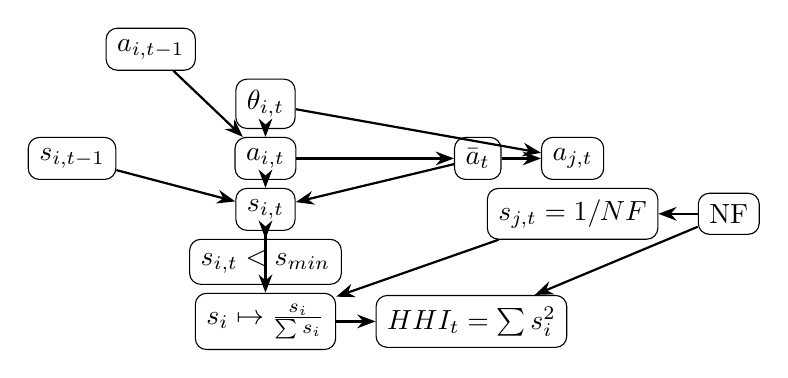
\begin{tikzpicture}[
    node distance=.1cm and 0.5cm,
    every node/.style={draw, rounded corners, minimum height=1.2em, inner sep=4pt, align=center},
    arrow/.style={-{Stealth}, thick}
    ]

    % Nodes
    \node (theta)        {$\theta_{i,t}$};
    \node (ai_tm1)       [above left=of theta] {$a_{i,t-1}$};
    \node (ai_t)         [below=of theta] {$a_{i,t}$};
    \node (si_tm1)       [left=1.5cm of ai_t] {$s_{i,t-1}$};
    \node (abar_t)       [right=2cm of ai_t] {$\bar{a}_t$};
    \node (si_t)         [below=of ai_t] {$s_{i,t}$};
    \node (exit)         [below=of si_t] {$s_{i,t} < s_{min}$};

    \node (aj_t)         [right=of abar_t] {$a_{j,t}$};
    \node (sj_t)         [below=of aj_t] {$s_{j,t} = 1/NF$};

    \node (norm_s)       [below=of exit] {$s_i \mapsto \frac{s_i}{\sum s_i}$};
    \node (HHI_t)        [right=of norm_s] {$HHI_t = \sum s_i^2$};

    \node (NF)           [right=of sj_t] {NF};

    % Arrows
    \draw[arrow] (ai_tm1) -- (ai_t);
    \draw[arrow] (theta) -- (ai_t);
    \draw[arrow] (ai_t) -- (abar_t);
    \draw[arrow] (si_tm1) -- (si_t);
    \draw[arrow] (ai_t) -- (si_t);
    \draw[arrow] (abar_t) -- (si_t);
    \draw[arrow] (si_t) -- (exit);

    \draw[arrow] (abar_t) -- (aj_t);
    \draw[arrow] (theta) -- (aj_t);
    \draw[arrow] (NF) -- (sj_t);
    \draw[arrow] (NF) -- (HHI_t);
    \draw[arrow] (si_t) -- (norm_s);
    \draw[arrow] (sj_t) -- (norm_s);
    \draw[arrow] (norm_s) -- (HHI_t);

    % Optional: Labels or braces could be added if needed
  \end{tikzpicture}
}
\end{frame}
\begin{frame}[label={sec:org0e6eba3},fragile]{Sequence of events}
 At time \(t = 0\), there are \(NF\) identical incumbent firms with equal \(a_{i,t=0}\) and \(s_{i,0}\).
At each time step \(t = 1, 2, \ldots, T\):
\begin{enumerate}
\item Firms learn (updates (\(a_{i}\))
\item Firms computes market share (updates \(s_{i}\))
\item Market concentration index (\(HHI\)) is computed
\item Firms exits the market if \(s_{i} < s_{min}\)
\item Firms enter to keep \(NF\) firms in the market
\item Incumbents variables (\(a_{j}\), \(s_{j}\)) are set
\item Market shares are re-scaled proportionally to ensure \(\sum s_{i} = 1\)
\end{enumerate}
\begin{block}{Model logical order (later)}
The exit-entry process is time-coordinated during each simulated time step by the technical variable \texttt{exit\_entry}: \texttt{HHI} > \texttt{exit\_decision} > \texttt{s} rescaling
\end{block}
\end{frame}
\begin{frame}[label={sec:org7caa6d1}]{Parameters and initial values}
\begin{table}[htbp]
\caption{Baseline parameters}
\centering
\begin{tabular}{ccc}
\hline
 & Desc & Value\\
\hline
\(\eta\) & Innovation opportunity support & 0.3\\
\(\beta_{1}, \beta_{2}\) & beta distribution parameters & 1.0; 5.0\\
\(A\) & replicator dynamics intensity & 1\\
\(s_{min}\) & minimum market share to not exit & 0.01\\
\(NF\) & number of firms & 10\\
\hline
\(a_{i}_{}\) & Initial Firm-level productivity & 1.0\\
\(s_{i}\) & Initial Firm market-share & \(1/NF\)\\
\hline
\end{tabular}
\end{table}
\end{frame}
\begin{frame}[label={sec:orgd060fbb}]{Model structure and data organization II}
\begin{figure}[htbp]
\centering
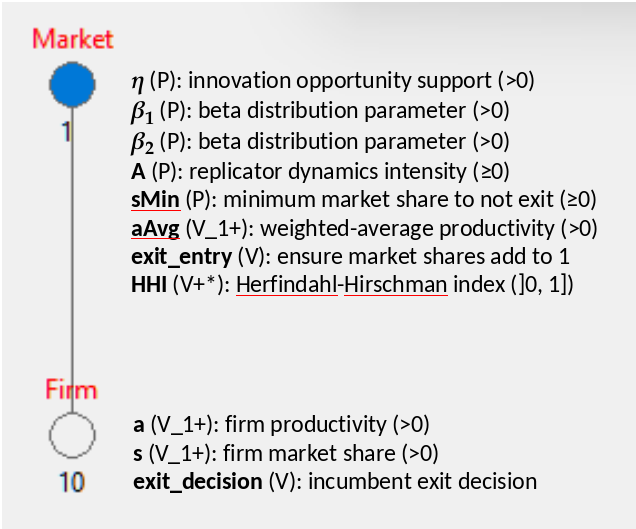
\includegraphics[clip,trim=0 0 0 0,width=.8\textwidth,height=.75\textheight]{figs/Structure_Industry_LSD.png}
\caption{Structure of industry model}
\end{figure}
\end{frame}
\begin{frame}[label={sec:orgd9c21f3}]{Memo: Equations}
\[ \begin{array}{lrl}
\mbox{Idiosyncratic learning process:} & a_{i,t} = &a_{i,t-1}\cdot (1 + \theta_{i,t})\\
\mbox{Learning shocks} & \theta_{i,t} \sim  & Beta(\beta_1, \beta_2)\\
\mbox{Market selection} & s_{i,t} =  & s_{i,t-1} \cdot \left( 1 + A\cdot\frac{a_{i,t} - \bar{a}_{t}}{\bar{a}_{t}}\right) \\
\mbox{Average productivity} & \bar{a}_{t} =  & \sum_{i=1}^{NF} s_{i, t-1}\cdot a_{i,t} \\
\mbox{Exit condition} & s_{i,t} < & s_{min}\\
\mbox{Entrant productivity} & a_{j,t} =&  \bar{a}_{t}\cdot (1 + \theta_{i,t})\\
\mbox{Entrant market-share} & s_{j,t} =& 1/NF \\
\mbox{Market concentration index} & HHI_{t} =& \sum_{i=1}^{NF} (s_{i})^2 \\
\mbox{Market-share adjustment} &  s_{i} \mapsto & s_{i}\cdot \frac{1}{\sum_{i=1}^{NF} s_{i}} \Rightarrow \sum_{i=1}^{NF} s_{i} = 1 \\
\mbox{Fixed number of firms} & \#\{1, \ldots, n\} =& NF
\end{array}\]
\end{frame}
\begin{frame}[label={sec:org0403772},fragile]{Firm-level productivity (\(a_{i}\)\textsubscript{nil})}
 \begin{equation}
a_{i,t} = a_{i,t-1}\cdot (1 + \theta_{i,t})
\end{equation}

\begin{minted}[]{cpp}
EQUATION("a")
// Firm knowledge/productivity
v[0] = CURRENT;
v[1] = V("eta");
v[2] = V("beta1");
v[3] = V("beta2");
v[4] = beta(v[2], v[3]);
v[5] = v[0] * (1 + v[1] * v[4]);
RESULT(v[5])
\end{minted}
\end{frame}
\begin{frame}[label={sec:org558b14b},fragile]{Market-share (\(s_{i}\))}
 \begin{equation}
s_{i,t} = s_{i,t-1} \cdot \left( 1 + A\cdot\frac{a_{i,t} - \bar{a}_{t}}{\bar{a}_{t}}\right)
\end{equation}


\begin{minted}[]{cpp}
EQUATION("s")
// Firm size/market share
v[0] = CURRENT;
v[1] = V("A");
v[2] = V("a");
v[3] = V("aAvg");
v[4] = (v[2] - v[3])/v[3];
v[5] = v[0] * (1 + v[1] * v[4]);
RESULT(v[5])
\end{minted}
\end{frame}
\begin{frame}[label={sec:orge208efa},fragile]{Exit condition}
 \begin{minted}[]{cpp}
EQUATION("exit_decision")

v[0] = V("s"); v[1] = V("sMin");
// update entrant firm productivity and market share
if (v[0] < v[1]) {
  v[2] = V("eta"); v[3] = V("beta1"); v[4] = V("beta2");
  v[5] = beta(v[3], v[4]);
  v[6] = V("aAvg");
  v[7] = v[6] * (1 + v[2] * v[5]);
  WRITE( "a", v[7] );
  WRITE( "s", 1 / COUNT( "Firm" ) );
}
RESULT(0)
\end{minted}
\end{frame}
\begin{frame}[label={sec:org7e43ad3},fragile]{Market-level Productivity (Weighted) Average (\(\bar{a_{t}}\))}
 \begin{equation}
\bar{a}_{t} =  \sum_{i=1}^{NF} s_{i, t-1}\cdot a_{i,t}
\end{equation}


\begin{minted}[]{cpp}
EQUATION( "aAvg" )
// Mean knowledge/productivity

v[0] = 0;        // accumulator
CYCLE(cur, "Firm") {
  v[1] = VLS( cur, "s", 1 );
  v[2] = VS( cur, "a" );
  v[3] = v[1] * v[2];
  v[0] += v[3] ;
}
RESULT( v[0] )
\end{minted}
\end{frame}
\begin{frame}[label={sec:org9463746},fragile]{Entry-Exit condition}
 \begin{minted}[]{cpp}
EQUATION( "exit_entry" )
// Trigger market-wise exit-entry dynamics and re-scale shares
V( "HHI" ); // first, compute HH index before exits

// second, ensure firms have decided on exit
CYCLE(cur, "Firm") {VS( cur, "exit_decision" );}

v[0] = 1 / SUM( "s" ); // factor to scale back to sum = 1
CYCLE(cur, "Firm") { // third, rescale market shares after exits
  v[1] = VS( cur, "s" );
  v[2] = v[0] * v[1];
  WRITES( cur, "s", v[2]);
}
RESULT( SUM("s") )
\end{minted}
\end{frame}
\begin{frame}[label={sec:orgcf60d8c},fragile]{Herfindahl-Hirschman concentration index (\(HHI\))}
 \begin{equation}
HHI_{t} = \sum_{i=1}^{NF} (s_{i})^2
\end{equation}


\begin{minted}[]{cpp}
EQUATION( "HHI" )
// Herfindahl-Hirschman concentration index
v[0] = WHTAVE( "s", "s" );
RESULT( v[0] )
\end{minted}
\begin{block}{Note on WHTAVE(LS)}
\texttt{WHTAVE} (weighed average, not used here in the strict sense) computes the sum of \(s\times s\) over every firm
\end{block}
\end{frame}
\begin{frame}[label={sec:org39ce6a5},fragile]{Initialization I}
 Firm-level initialization can be set for every \(NF\) objects on the LSD browser.
The same applies for every other initial condition.

In the following slide, we will see an alternative way in which we control some few parameters and create \(NF-1\) copies of a example object.

\begin{minted}[]{cpp}
ADDNOBJ_EX("TypeOfAgent", number, *pointer);
\end{minted}
\begin{block}{Semi-automated initialization and sensitivity analysis}
By doing this, we automate the model initialization to test different model configurations (next lecture)
\end{block}
\end{frame}
\begin{frame}[label={sec:org5014c5f},fragile]{Initialization II}
 \begin{minted}[]{cpp}
EQUATION( "init" )
PARAMETER;                  // turn into parameter (run once)
// finds the agent on memory
cur = SEARCH( "Market" ); cur1 = SEARCHS(cur, "Firm" );

v[0] = V("A0"); // We define
v[1] = V("Nfirm"); // We define
v[2] = 1 / v[1]; // Fair share
// Overwrites the lag 1 of "a" to v[0] at time 1
WRITELLS(cur1, "a", v[0], 1, 1);
WRITELLS(cur1, "s", v[2], 1, 1);
// Adds N - 1 copies of cur1 agent located under cur
ADDNOBJ_EXS(cur, "Firm", v[1] - 1, cur1);
RESULT( 1 )
\end{minted}
\end{frame}
\section{Session 3}
\label{sec:org37d8a22}

\begin{frame}[label={sec:org7ea30f9}]{Where are we are where are we going?}
\begin{description}
\item[{Session I}] Basics of LSD and small models implementation
\item[{Session II}] Presentation of the Industry model and implementation
\item[{Session III (Today)}] Q\&A, bug fixes, and analysis of results and Monte Carlo Experiment
\end{description}
\end{frame}
\begin{frame}[label={sec:org580595d}]{Analyzing the model results}
\begin{itemize}
\item After a successful simulation run, in \alert{Browser} click on menu \alert{Data > Analysis of Results}
\item To analyze the \emph{saved} data time series, select the desired variables from the \alert{Series available} list to include them in the \alert{Series selected} list
\item Click on \alert{Plot} button to show the selected variable(s) time series plot
\item Click on \alert{Statistics} button to show the selected time series descriptive statistics in \alert{LSD Log}
\item Plots and analysis data can be \emph{saved} pressing the \alert{Save Plot} and \alert{Save Data} buttons
\end{itemize}
\end{frame}
\begin{frame}[label={sec:org86cb44e}]{Exploring the single run results}
\begin{figure}[ht]
    % First row: Market-level data
    \begin{subfigure}{0.48\textwidth}
        \centering
        \includesvg[width=\linewidth, height=.3\textheight]{./figs/single_avg_log_productivity.svg}
        \caption{Average log-productivity ($a$)}
        \label{fig:avg_prod}
    \end{subfigure}
    \hfill
    \begin{subfigure}{0.48\textwidth}
        \centering
        \includesvg[width=\linewidth, height=.3\textheight]{./figs/single_firm_log_productivity.svg}
        \caption{Firm log-productivity ($a$)}
        \label{fig:firm_prod}
    \end{subfigure}

    % Second row: Firm-level data
    \begin{subfigure}{0.48\textwidth}
        \centering
        \includesvg[width=\linewidth, height=.3\textheight]{./figs/single_HHI.svg}
        \caption{Herfindahl-Hirschman Index (HHI)}
        \label{fig:hhi}
    \end{subfigure}
    \hfill
    \begin{subfigure}{0.48\textwidth}
        \centering
        \includesvg[width=\linewidth, height=.3\textheight]{./figs/single_firm_market_share.svg}
        \caption{Firm market share ($s$)}
        \label{fig:market_share}
    \end{subfigure}
    \label{single-run-industry}
\end{figure}
\end{frame}
\begin{frame}[label={sec:orgbb1502b},fragile]{Activity I}
 \begin{enumerate}
\item Show that average productivity (\texttt{aAvg}) is always between than maximum and minimum productivities
\item Check that the total market share of firms is constant and equal to 1
\item Increase (1) the number of firms to 150, (2) the exit threshold \texttt{sMin} to 0.001, and the number of simulation steps.
\item Run and analyze the results. What are the main differences?
\item Using this new configuration, produce a \alert{histogram} of the firm log-size distribution at \(t = 200\)
\end{enumerate}
\end{frame}
\begin{frame}[label={sec:org2f3d552}]{Histogram of firm log-size distribution (\(t = 200\))}
\begin{center}
\includesvg[width=.9\linewidth]{./figs/150_firms_log_size_histogram}
\end{center}
\end{frame}
\begin{frame}[label={sec:org5fcbc00}]{A simple Monte Carlo experiment I}
\begin{enumerate}
\item Close Analysis of Results window
\item Re-open the baseline configuration
\item Set the simulation runs to \alert{20} (\alert{Run > Simulation})
\item Save as a new configuration
\item Run the new configuration (\alert{Run > Run})
\item Choose \alert{Data > Analysis of MC Experiment}, accept using last results, and mark to create \alert{Average} and \alert{Maximum and minimum} series, and to include confidence intervals
\item Analyze the Monte Carlo experiment results
\end{enumerate}
\end{frame}
\begin{frame}[label={sec:org89959de}]{A simple Monte Carlo experiment II}
\begin{center}
\includesvg[width=.9\linewidth]{./figs/HHI_MC}
\end{center}
\end{frame}
\begin{frame}[label={sec:org47ff5fa}]{Activity II}
\begin{enumerate}
\item Show the max-min intervals for the average log-productivity (\alert{aAvg}) and the \alert{HHI} in the MC experiment
\item Why the MC confidence width is not comparable for the two variables?
\item Show the distribution of the productivity (\alert{a}) considering all MC runs (tip: select \alert{Keep original series in Monte Carlo options})
\item The Monte Carlo analysis uncovers a potential problem with this simplified version of the model, try to identify it, and to reason if it can invalidate the results obtained
\end{enumerate}
\end{frame}
\section{Bonus}
\label{sec:org8d25251}

\begin{frame}[label={sec:org4ea45d2}]{Model sensitivity to parameters}
How do parameters and initial conditions \alert{jointly} affect variables?

\begin{itemize}
\item The most common approach is to perform a one-variable at a time change
\begin{itemize}
\item In this small-scale model, we can play with different parameters and check
\end{itemize}
\item However, even with this small parametric space, the number of combinations can get quickly large
\item We will briefly check some Design of Experiments Techniques that helps with this situations
\end{itemize}
\end{frame}
\begin{frame}[label={sec:orgf583430}]{Sensitivity analysis}
Sensitivity analysis requires many steps:

\begin{enumerate}
\item Screening: Filter down unimportant factors (elementary effects)
\item Select a \alert{Design of Experiments} (DoE) strategy
\item Evaluate multiple runs per configuration
\item If required, fit a \alert{meta-model}
\item Compute the sensitivity analysis \alert{statistics}
\item Explore the \alert{response surfaces}
\end{enumerate}

\alert{Good news:} LSD (+R) can handle this through a NNF approach
\begin{block}{Note on screening}
As the model is small, we will skip screening and jump directly to metamodels
\end{block}
\end{frame}
\begin{frame}[label={sec:org657924d}]{Parametric space}
\begin{center}
\begin{tabular}{ccccc}
\hline
 & Desc & Baseline & Min & Max\\
\hline
\(\eta\) & Innovation opportunity support & 0.3 & 0.0 & 0.7\\
\(\beta_{1}, \beta_{2}\) & beta distribution parameters & 1.0; 5.0 & 1; 3 & 3;10\\
\(A\) & replicator dynamics intensity & 1 & 0.2 & 5\\
\(s_{min}\) & minimum market share to not exit & 0.01 & 0.0001 & 0.01\\
\(NF\) & number of firms & 10 & 10 & 350\\
\hline
\end{tabular}
\end{center}
\begin{block}{Monte Carlo vs Near Orthogonal Latin Hypercube}
\begin{itemize}
\item All combinations possible (MC): 64 (x 5)
\item NOLH: 43 (x 5)
\end{itemize}
\end{block}
\end{frame}
\begin{frame}[label={sec:org78d14f0}]{Exploring the industry model}
Load \href{Industry\_SummerSchool/R/data/Sim-Sobol.lsd}{R/data/Sim-Sobol.lsd} file in LSD
\begin{enumerate}
\item This is a copy of \href{Industry\_SummerSchool/Sim1.lsd}{Sim1.lsd} with 5 simulation runs
\end{enumerate}
\begin{enumerate}
\item Load sensitivity analysis configuration (\alert{File > Load sensitivity\ldots{}}) and choose \href{Industry\_SummerSchool/R/Sim-Sobol.sa}{R/Sim-Sobol.sa}
\item Set the DoE (\alert{Data > Sensitivity Analysis > NOHL sampling})
\begin{enumerate}
\item Select \alert{Extended number of samples}, hit \alert{OK} and accepts the default
\end{enumerate}
\item Run a \alert{parallel batch} (Run > Parallel Batch) to produce the results files (accept the defaults)
\item Let's jump into R(studio) and create a project under the \alert{R} folder
\item Select the \alert{sobol-SA.R} and hit source
\end{enumerate}
\begin{block}{Before checking the results}
Which parameters do you expect to most influence \alert{HHI}? What about \alert{aAvg}?
\end{block}
\end{frame}
\begin{frame}[label={sec:orgd89c35b}]{Sobol decomposition indexes (HHI)}
\begin{center}
\includegraphics[height=.875\textheight,page=4]{./Industry_SummerSchool/R/data/Sim-Sobol_kriging_HHI.pdf}
\end{center}
\end{frame}
\begin{frame}[label={sec:org2990028}]{Meta-model response I}
\begin{center}
\includegraphics[height=.85\textheight,page=5]{./Industry_SummerSchool/R/data/Sim-Sobol_kriging_HHI.pdf}
\end{center}
\end{frame}
\begin{frame}[label={sec:org58979f0}]{Meta-model response II}
\begin{center}
\includegraphics[height=.85\textheight,page=6]{./Industry_SummerSchool/R/data/Sim-Sobol_kriging_HHI.pdf}
\end{center}
\end{frame}
\begin{frame}[label={sec:orga4659fe}]{Meta-model response III}
\begin{center}
\includegraphics[height=.85\textheight,page=7]{./Industry_SummerSchool/R/data/Sim-Sobol_kriging_HHI.pdf}
\end{center}
\end{frame}
\begin{frame}[label={sec:org1eb72f8},fragile]{Bonus Activity}
 \begin{itemize}
\item In the Rscript, uncomment \texttt{varName   <- "aAvg"} and source the file again
\item Open the resulting PDF file
\item Analyze the results and contrast with your expectations
\item What are the economic intuition associated with these parameters?
\end{itemize}
\end{frame}
\begin{frame}[label={sec:org5eec1cb}]{Phew!}

Our papers are available at:

\faNewspaper\ \texttt{http://www.lem.sssup.it/wplem.html}\\

You can reach me at:

\faEnvelope\ \texttt{gpetrinidasilveira@gmail.com} \\
\faGithub\ \texttt{github.com/gpetrini} \\
\faOrcid & \texttt{https://orcid.org/0000-0002-3523-9826} \\

\\\Huge{Thank you!}
\end{frame}
\end{document}
